\subsubsection{ResNet}\label{resnet}
The Residual Network architecture (ResNet) was first introduced by \citep{he2015deep} in their paper ``Deep Residual Learning for Image Recognition''. This marked a big advancement in deep learning for computer vision, as previous model architectures did not have the ability to effectively scale with more layers. These models would, among other issues, run into a vanishing or exploding gradient problem, making deeper layers less usefull and impacting performance. To combat this, ResNet introduces a solution using residual blocks, as shown in Figure~\ref{fig:residualBlock}. The input X goes through two paths. One is called a skip connection and carries the original input to a junction point. The other carries the input through multiple convolutional layers to process it. Following the first layer, the input is passed through a ReLu function, introducing non-linearity to the model. Then it is passed trough a second convolutional layer, which returns a residual function. In the end, the learned residual function is added to the original input.
\begin{figure}[ht]
    \centering
    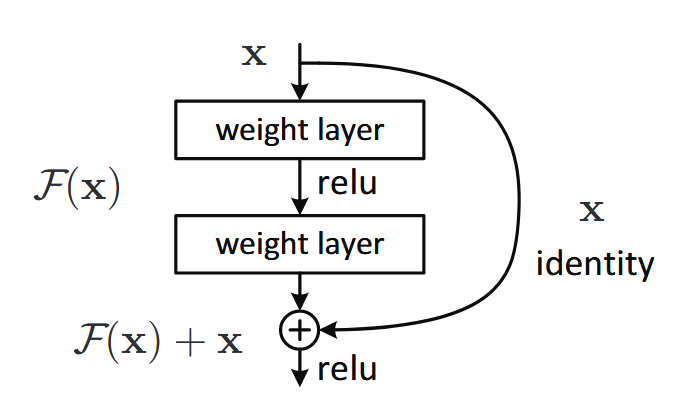
\includegraphics[width=0.7\textwidth]{figures/ResidualBlock.png}
    \caption{Residual Block as outlined by \citeauthor{he2015deep}.}\label{fig:residualBlock}
\end{figure}

\subsubsubsection{ResNet18 and ResNet32:}\label{resnet18}
Using the block shown in Figure~\ref{fig:residualBlock}, the researchers built two networks, that are now commonly used. ResNet18, containing 18 and ResNet32, containing 32 layers, made of these two-layer residual blocks. These networks are designed for simpler tasks and limited training resources. They offer great performance relative to their size.

\begin{figure}[ht]
    \centering
    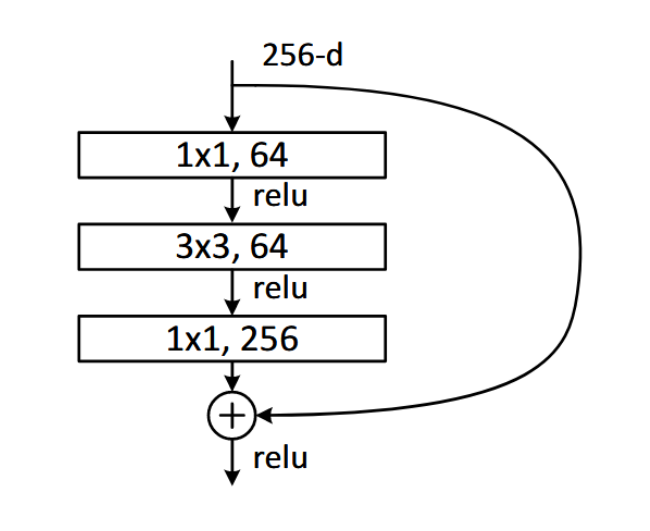
\includegraphics[width=0.6\textwidth]{figures/BottleNeckBlock.png}
    \caption{Bottleneck Block as outlined by \citeauthor{he2015deep}.}\label{fig:bottleneckBlock}
\end{figure}

\subsubsubsection{ResNet50, ResNet101 and ResNet152:}\label{resnet152}
In order to further upscale this technology, the researchers introduced a modification to the two-layer structure. As seen in Figure~\ref{fig:bottleneckBlock}, the researchers created a bottleneck block. This block features two convolutional layers with a 1$\times$1 convolution and a middle layer with a  3$\times$3 convolution. The first layer down scales the input, which is then forwarded to the next layer with a 3$\times$3 convolution. This middle layer is the core of the bottleneck block, where the actual feature extraction happens. Then the third layer upscales the input back to its original size and returns the output for the block. These Models work well for large and complicated datasets but are more computationally demanding than their two-layer counterparts. 